%
% packages & config
%

\documentclass[utf8,english]{gradu3}

\usepackage{graphicx}
\usepackage{csquotes}
\usepackage{amsmath,amssymb,amsthm}
\usepackage{biblatex}
\usepackage[bookmarksopen,bookmarksnumbered,linktocpage]{hyperref}

\usepackage{tikz}
\usetikzlibrary{arrows.meta}
\tikzset{>=latex}
\usetikzlibrary{3d}
\usetikzlibrary{calc}

% the default LaTeX font for \mathcal
% (gradu3.cls contains font config that makes it unreadable)
\DeclareMathAlphabet{\mathcal}{OMS}{cmsy}{m}{n}

%
% metadata
%

\addbibresource{sources.bib}

\title{Discrete Exterior Calculus and Exact Controllability for Time-Harmonic Acoustic Wave Simulation}
\translatedtitle{Diskreetti ulkoinen laskenta ja kontrollimenetelmä aikaharmonisessa akustiikkasimulaatiossa}
\author{Mikael Myyrä}
\contactinformation{\texttt{mikael.b.myyra@jyu.fi}}
\supervisor{Sanna Mönkölä, Tuomo Rossi, Jonni Lohi}
\studyline{Teknis-matemaattinen mallintaminen (TODO: translate)}
\tiivistelma{-}
\abstract{-}
\avainsanat{
diskreetti ulkoinen laskenta,
kontrollimenetelmä,
akustiikka,
simulointi
}
\keywords{
discrete exterior calculus,
exact controllability,
acoustics,
simulation
}

%
% begin document
%

\begin{document}

\maketitle

% table of contents generates slightly overfull hboxes for some reason,
% suppress those errors with a bit of fuzz
\hfuzz=1.5pt
\mainmatter
\hfuzz=0pt


\chapter{Introduction}



\chapter{Model}

The phenomenon we wish to simulate is the scattering
of acoustic waves by a sound-soft obstacle (TODO: what does sound-soft mean).
We consider acoustic waves described by the differential equation

\begin{equation}
  \frac{\partial^2 \phi}{\partial t^2} - c^2 \nabla^2\phi = 0
\end{equation}

where $\phi$ is a velocity potential and $c$ is the speed of wave propagation.
This equation is equivalent to the first-order system

\begin{equation}\label{wave1stOrd}
  \begin{cases}
    \frac{\partial p}{\partial t} - c^2\nabla \cdot \mathbf{v} = 0 \\
    \frac{\partial \mathbf{v}}{\partial t} - \nabla p = 0 \\
  \end{cases}
\end{equation}

where $p = \frac{\partial \phi}{\partial t}$ is acoustic pressure
and $\mathbf{v} = \nabla \phi$ is the velocity
of particles perturbed by the wave.

The system \eqref{wave1stOrd} applies within the spatial domain $\Omega$
and the time domain $[0, T]$.
We model the scattering obstacle by excluding its interior from $\Omega$
and applying an incoming wave $\phi_{inc}$ on its boundary $\Gamma_{sca}$
as a Dirichlet boundary condition

\[
  \begin{cases}
    p = \frac{\partial \phi_{inc}}{\partial t} \\
    \mathbf{v} = \nabla \phi_{inc} \\
  \end{cases}
  \quad \text{in } \Gamma_{sca} \times [0, T].
\]

On the outer boundary of the domain $\Gamma_{ext}$
we model the uninterrupted propagation of waves past the boundary
with a first-order absorbing Engqvist-Majda boundary condition
\parencite{engquist_absorbing_1977}

\[
  \frac{1}{c}\frac{\partial\phi}{\partial t} + \mathbf{n} \cdot \nabla\phi = 0
  \quad \text{in } \Gamma_{ext} \times [0, T].
\]


TODO: maybe the boundary conditions would be better explained
in the experiments chapter?
Possibly remove this chapter altogether
and explain the model in parts elsewhere



\chapter{Discrete Exterior Calculus}

Discrete Exterior Calculus (DEC),
originally developed by Desbrun et al. \parencite*{desbrun_discrete_2005},
is a discretization method for differential equations
based on the exterior calculus of differential forms.
This chapter gives a brief introduction to the mathematical concepts
underlying the method, followed by a description of the DEC itself
and a DEC discretization of our acoustics equations.
The reader is assumed to be familiar with linear algebra and vector calculus.


\section{Differential forms and the continuous exterior calculus}

This section is meant as a somewhat informal and intuitive introduction
to differential forms, summarizing relevant sections of
\parencite{blair_perot_differential_2014} and \parencite{crane_digital_2013}.
For a more formal and comprehensive approach to the topic,
see a textbook on differential geometry such as \parencite{lee_introduction_2012}
or \parencite{abraham_manifolds_2012}.


\subsection{Differential forms}

Notationally, a differential form looks like an \textit{integrand},
e.g. the $dx$ in $\int dx$ or the $5\,dx\,dy$ in $\iint 5\,dx\,dy$.
Indeed, the things we integrate are all technically differential forms.
However, this seems rather abstract.
Are these objects meaningful outside of integration,
and if so, what do they do?
This section looks at differential forms as functions,
taking inspiration from \parencite{crane_digital_2013}.

Differential forms are in many ways analogous to vectors.
To illustrate the similarities and differences,
consider the dot product operation
for two vectors in linear algebra.
Expressed in matrix form, the dot product between vectors
$\mathbf{a} = (a_1, \dots, a_n)^T$ and $\mathbf{b} = (b_1, \dots, b_n)^T$
is

\[
  \mathbf{a} \cdot \mathbf{b} = \mathbf{a}^T \mathbf{b}
  = \begin{bmatrix}
    a_1 & \dots & a_n
  \end{bmatrix}
  \begin{bmatrix}
    b_1 \\ \vdots \\ b_n
  \end{bmatrix}.
\]

The dot product measures the length of $\mathbf{b}$ in the direction of $\mathbf{a}$,
and to do this, $\mathbf{a}$ is transposed into a \textit{row vector}.
This row vector can be thought of as a function
that takes a vector and measures it along $\mathbf{a}$,

\[
  \alpha(\mathbf{b}) = \mathbf{a}^T \mathbf{b}.
\]

In the language of differential forms,
a function like this is called a \textit{1-form},
because it takes a single vector as its parameter
and computes its length along one dimension.

We can also measure higher-dimensional quantities.
A 2-form is a function that takes two vectors,
which define a parallelogram,
and computes the area of this parallelogram
when projected onto a plane.
Similarly, 3-forms measure the volumes of parallelepipeds
defined by three vectors, and so on for higher dimensions.
Additionally, we can define 0-forms
as objects that take zero vectors as input and return a measurement,
making them equivalent to scalar fields.

For forms of dimension 2 and above, we also need to consider
the notion of \textit{signed} areas and volumes.
Much like how the vector cross product flips its direction
depending on whether its arguments come in clockwise or counterclockwise order,
a differential form's output will change its sign
if any two of its arguments are exchanged.
The sign is a measurement of the given volume's \textit{orientation}:
clockwise or counterclockwise for 2D areas,
right-handed or left-handed basis for 3D volumes, etc.
This is why differential forms are formally defined as \textit{antisymmetric tensors}
-- they're multilinear functions on vectors (i.e. tensors)
which change sign when arguments are exchanged (i.e. they are antisymmetric).

\subsection{Basis forms}

Like vectors, differential forms also form a vector space,
meaning they can be expressed as linear combinations of basis vectors.
In $\mathbb{R}^3$, with axes labeled $x$, $y$, and $z$,
the corresponding basis 1-forms are called $dx$, $dy$, and $dz$.

Higher-dimensional forms also have this vector space structure,
but defining a basis for them is not quite as straightforward.
The issue is that $n$-forms measure $n$-dimensional geometric objects
which require $n$ different vectors to define.
Thus, to define an $n$-form we need a formal way to combine
measurements in $n$ different directions.
The operator which does this is called the \textit{exterior product}.

\subsection{Exterior product}

You may recall from linear algebra that the signed area of a parallelogram
defined by two vectors $u,v$ in $\mathbb{R}^3$ is computed
by the cross product $u \times v$.
Similarly, the volume of a parallelepiped defined by three vectors $u,v,w$
is computed by the triple product $(u \times v) \cdot w$,
and in general the volume spanned by $n$ vectors $v_1, \dots, v_n$
is the determinant
\[
  \det \begin{bmatrix}
    v_1, \dots, v_n
  \end{bmatrix}.
\]

The analogous operation for differential forms is called the
\textit{exterior product} or \textit{wedge product} $\wedge$,
which takes a $k$-form $\alpha$ and a $j$-form $\beta$
and produces a $(k+j)$-form which measures volumes spanned by
$\alpha$ and $\beta$ combined.
For instance, if $\alpha$ and $\beta$ are both 1-forms,
$\alpha \wedge \beta$ is a 2-form which measures parallelograms
in the plane spanned by $\alpha$ and $\beta$.

Depending on the dimension of forms being multiplied,
the wedge product's sign may change
when the order of its arguments is flipped. Specifically,
\[
  \alpha \wedge \beta = (-1)^{kj} \beta \wedge \alpha.
\]
Additionally, the wedge product is associative, meaning
\[
  (\alpha \wedge \beta) \wedge \gamma = \alpha \wedge (\beta \wedge \gamma).
\]

These three properties (addition of dimensions, antisymmetry, and associativity)
are enough to define the wedge product abstractly in all dimensions.
In practice, what this operation looks like depends on the dimension of its operands
in the way already mentioned -- the wedge product of two 1-forms in 3D space
behaves like the vector cross product,
and the wedge product of three 1-forms (really a 2-form and a 1-form)
behaves like the triple product.
Additionally, since a 0-form is just a scalar,
the wedge product of a 0-form with anything behaves like scalar multiplication.

To give a specific example, consider two vectors $u,v$ in $\mathbb{R}^3$
and two 1-forms $\alpha, \beta$. The wedge product
\[
  \alpha \wedge \beta (u,v) = \alpha(u)\beta(v) - \alpha(v)\beta(u),
\]
which behaves like the cross product between the vectors
$(\alpha(u), \alpha(v))$ and $(\beta(u), \beta(v))$.

The 1-form wedge product can be visualized as combining two vectors
into a single oriented parallelogram,
or in other words, two basis elements of a line
into a basis element of a plane.
Similarly, further wedge products add on more basis elements,
producing higher-dimensional oriented volumes.

\begin{figure}[h]
  \centering
  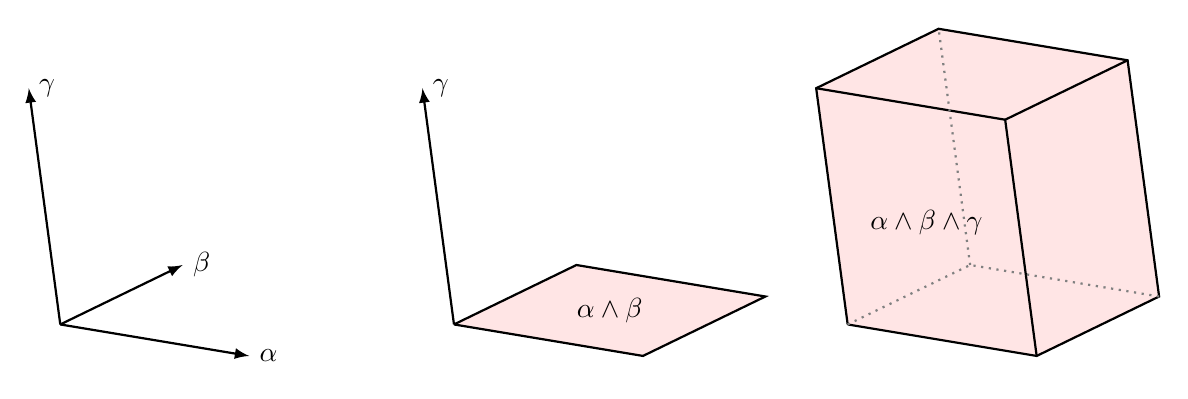
\begin{tikzpicture}[scale=2, thick]
    \coordinate (x) at (1.2, -0.2, 0);
    \coordinate (z) at (0.2, -0.2, -1.5);
    \coordinate (y) at (-0.2, 1.5, 0);
    \draw[->] (0,0,0) -- (x);
    \draw[->] (0,0,0) -- (z);
    \draw[->] (0,0,0) -- (y);
    \node[anchor=west] at (x) {$\alpha$};
    \node[anchor=west] at (z) {$\beta$};
    \node[anchor=west] at (y) {$\gamma$};

    \begin{scope}[xshift=2.5cm]
      \coordinate (x) at (1.2, -0.2, 0);
      \coordinate (z) at (0.2, -0.2, -1.5);
      \coordinate (y) at (-0.2, 1.5, 0);
      \draw[fill=red!10] (0,0,0) -- (x) -- ($(x) + (z)$) -- (z) -- (0,0,0);
      \draw[->] (0,0,0) -- (y);
      \node at ($0.5*(x) + 0.5*(z)$) {$\alpha \wedge \beta$};
      \node[anchor=west] at (y) {$\gamma$};
    \end{scope}

    \begin{scope}[xshift=5cm]
      \coordinate (x) at (1.2, -0.2, 0);
      \coordinate (z) at (0.2, -0.2, -1.5);
      \coordinate (y) at (-0.2, 1.5, 0);
      \fill[fill=red!10] (0,0,0) -- (x) -- ($(x) + (z)$) -- ($(x) + (y) + (z)$) -- ($(y) + (z)$) -- (y) -- (0,0,0);
      \draw (0,0,0) -- (x) -- ($(x) + (z)$) -- ($(x) + (y) + (z)$) -- ($(y) + (z)$) -- (y) -- (0,0,0);
      \draw (x) -- ($(x) + (y)$) -- ($(x) + (y) + (z)$);
      \draw (y) -- ($(x) + (y)$);
      \draw[gray,dotted] (0,0,0) -- (z) -- ($(x) + (z)$);
      \draw[gray,dotted] (z) -- ($(z) + (y)$);
      \node at ($0.5*(x) + 0.5*(y)$) {$\alpha \wedge \beta \wedge \gamma$};
    \end{scope}
  \end{tikzpicture}
  \caption{Exterior products of 1-forms visualized as volumes.}
  \label{fig:wedge}
\end{figure}

Can't make forms of higher dimension than embedding space

Three basis planes in 3D

TODOs:
\begin{itemize}
  \item using forms interchangeably with their vector proxies
  \item integration (1-forms -> line integrals, 2-forms -> surface integrals etc.)
  \item exterior derivative
  \item Hodge star
  \item why this is useful: coordinate-free formulas (simplicity/conciseness),
    curved space, higher dimensional space
  \item manifolds?
  \item acoustics equations expressed with differential forms?
    or maybe that should go in section \ref{sec:dec_model}
  \item einstein summation notation? (explain it if I use it)
\end{itemize}


\section{Computation mesh}

The discrete spatial structure at the root of the DEC is the \textit{simplicial complex}:
essentially a mesh (in the computer graphics sense)
consisting of triangles in two dimensions,
tetrahedra in three dimensions, or \textit{$k$-simplices} in $k$ dimensions.
We will focus on the two-dimensional case here for illustration.
This section is based on \parencite{desbrun_discrete_2006}.


\subsection{Simplices}

A \textit{$k$-simplex} is the simplest type of $k$-dimensional element
in a polyhedral mesh, defined as
the convex hull of $k + 1$ geometrically distinct points.
In concrete terms, a 0-simplex is a single point,
a 1-simplex is a line segment, a 2-simplex is a triangle,
a 3-simplex is a tetrahedron, and so on.
In the context of a mesh, a 0-simplex is often called a \textit{vertex},
a 1-simplex an \textit{edge}, a 2-simplex a \textit{face},
and a $k$-simplex where $k > 2$ a \textit{volume} or \textit{$k$-volume}.

Every simplex with dimension $k > 0$
has a \textit{boundary} consisting of $(k-1)$-simplices.
For instance, every triangle (2-simplex) is bounded by three line segments (1-simplices),
and every line segment is bounded by two vertices.
Each $(k-1)$-simplex on the boundary of a $k$-simplex $\sigma_k$
is called a \textit{$(k-1)$-face} of $\sigma_k$.

We denote simplices by listing their vertices, e.g. a triangle
$\sigma_2 = \{v_0, v_1, v_2\}$.


\subsection{Simplicial complex}

A simplicial complex $\mathcal{K}$ is a set of simplices satisfying the rules

\begin{itemize}
  \item every face of every simplex in $\mathcal{K}$ is also in $\mathcal{K}$
  \item any two simplices in $\mathcal{K}$ either do not intersect at all
    or share an entire face.
\end{itemize}

In the case of a 2D triangle mesh, this means
that every edge and vertex of every triangle is also part of the complex,
and there are no overlapping triangles
or edges/vertices that aren't part of a triangle's boundary.

A similar complex could be defined without requiring
all its elements to be simplicial.
For instance, a rectilinear grid is a common such structure.
A complex like this is called a \textit{cell complex}
and its $k$-dimensional elements \textit{$k$-cells}.
A simplex is a special case of a cell,
and the concepts of boundary and face apply to all cells.
We will use a simplicial complex in this thesis,
however, non-simplicial cells become relevant in the \textit{dual mesh}
(section \ref{sec:dual_mesh}).


\subsection{Orientation of a simplex}

Much like how differential forms of dimension 2 and higher
have a notion of two distinct orientations,
which manifest themselves in the sign of measured volumes,
simplices with 2 or more vertices also have two possible orientations
depending on the order of the vertices.
For a line segment there are two possible ways to order its two vertices,
for a triangle there are three clockwise and three counterclockwise orderings,
and so on.

As part of the definition of our simplicial complex,
each simplex receives an orientation.
For reasons that will become clear when
we define the discrete exterior derivative in section \ref{sec:disc_ext_der},
every simplex also needs its boundary to match its orientation.
For a counterclockwise oriented triangle, for instance,
this means the boundary line segments must form
a counterclockwise circulation around the triangle.
Since a line segment is often part of two triangles with conflicting orientations,
the defined orientations cannot be consistent with every boundary.

To resolve inconsistent face orientations,
the \textit{boundary operator} $\partial$,
which takes a simplex and returns its faces,
must flip every face that doesn't match the desired orientation.
This is denoted as a multiplication by -1.
For example, the boundary of a counterclockwise oriented triangle $\{v_0, v_1, v_2\}$
with edges $\{v_0, v_1\}$, $\{v_1, v_2\}$, $\{v_0, v_2\}$ is
\[
  \partial \{v_0, v_1, v_2\} = \{v_0, v_1\} + \{v_1, v_2\} - \{v_0, v_2\}.
\]

\begin{figure}[h]
  \centering
  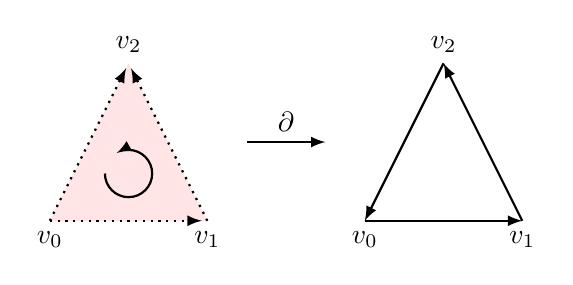
\begin{tikzpicture}
    \fill[fill=red!10] (-1,0) -- (1,0) -- (0,2);
    \draw[thick, dotted, -{>[sep=2pt]}] (-1,0) node[anchor=north]{$v_0$} -- (1,0);
    \draw[thick, dotted, -{>[sep=2pt]}] (1,0) node[anchor=north]{$v_1$} -- (0,2);
    \draw[thick, dotted, -{>[sep=2pt]}] (-1,0) -- (0,2) node[anchor=south]{$v_2$};
    \draw[thick, ->] (-0.3,0.6) arc (-180:120:0.3);

    \draw[thick, ->] (1.5, 1) -- node[anchor=south]{$\partial$} (2.5, 1);

    \draw[thick, ->] (3,0) node[anchor=north]{$v_0$} -- (5,0);
    \draw[thick, ->] (5,0) node[anchor=north]{$v_1$} -- (4,2);
    \draw[thick, ->] (4,2) node[anchor=south]{$v_2$} -- (3,0);
  \end{tikzpicture}
  \caption{
    \label{fig:triangle_boundary}
    Boundary of a triangle with inconsistently oriented faces.
  }
\end{figure}


\subsection{Chains and cochains}\label{sec:chains}

A \textit{$k$-chain} on a simplicial complex $\mathcal{K}$
is a set of real values associated with every $k$-simplex in $\mathcal{K}$.
Denoting the set of all $k$-simplices in $\mathcal{K}$ by $\mathcal{K}^k$
and its cardinality by $|\mathcal{K}^k|$,
a natural represenation for a chain is a $|\mathcal{K}^k|$-dimensional vector.
The space of all $k$-chains $\mathcal{C}_k$ is a vector space,
and the set of all $k$-simplices can be thought of as its basis.

Whereas a chain is analogous to a vector,
a \textit{cochain} is analogous to a differential form:
a linear function that takes a chain and ''measures'' it,
producing a real number.
A $k$-cochain $\omega^k$ has one linear operation for each $k$-simplex in $\mathcal{K}$,
matching the dimension of the corresponding $k$-chain $c_k$,
and the evaluation $\omega^k(c_k)$ behaves like an inner product between vectors.
Thus, a natural way to represent a cochain is a $|\mathcal{K}^k|$-dimensional \textit{row vector}.

This analogy with differential forms will be useful
when we define discrete forms in the next section.


\section{Discrete differential forms}

Equipped with an oriented simplicial complex,
we can begin to map differential forms and their operations onto it.
This section is based on \parencite{desbrun_discrete_2006},
\parencite{crane_digital_2013}, and \parencite{blair_perot_differential_2014}.


\subsection{Definition of discrete forms}

Recalling that differential forms can be integrated
over manifolds of matching dimension,
a natural way to map a continuous form to a discrete value on a simplex
is to integrate the form over that simplex.
In other words, given a differential $k$-form $\omega^k$
and $k$-simplex $\sigma_k$, we can get a scalar value $\widehat{\omega}^k$
associated with $\sigma_k$ by computing the integral

\[
  \widehat{\omega}^k = \int_{\sigma_k} \omega^k.
\]

This is a line integral over a line segment for 1-forms,
surface integral over a triangle for 2-forms,
volume integral over a tetrahedron for 3-forms, and so on.
Additionally, a 0-form (i.e. a scalar field)
integrated over a 0-simplex (i.e. a single point)
is the value of the form at that point.

Computing this integral for every $k$-simplex in a simplicial complex $\mathcal{K}$
produces a set of values associated with the $k$-simplices,
which can be interpreted as a chain or cochain.
Due to the analogous nature of differential forms and cochains
covered in section \ref{sec:chains},
the most fitting choice of interpretation here is a cochain.
This leads us to the following definition:

A discrete differential $k$-form on an oriented simplicial complex $\mathcal{K}$
is a $k$-cochain obtained by integrating a continuous $k$-form
over every $k$-simplex in $\mathcal{K}$.

A consequence of defining discrete forms as a single real value per simplex
is that vector-valued forms (1-forms and 2-forms in 3D)
lose information about their direction.
A line integral only records the component of the form tangential to the line,
discarding the orthogonal component,
and a surface integral is only affected by flux across the surface.
However, directions are not actually needed in most DEC computations.
If one is desired (e.g. for visualization),
it can be reconstructed from multiple nearby simplices via \textit{interpolation},
which will be covered in section \ref{sec:interpolation}.

TODO: that last paragraph is maybe a bit confusing,
can I word it better or move it somewhere else?
Could be best to just say this in the interpolation section
without alluding to it beforehand

The discrete equivalent of a differential form being a cochain,
the discrete versions of the operations of exterior calculus
are operations on cochains.

\subsection{Discrete exterior derivative}\label{sec:disc_ext_der}

Recall that the exterior derivative
is equivalent to the vector calculus operators
of gradient, curl, and divergence, depending on the dimension of the form.
The exterior derivative also increases the dimension of the form by one,
representing a shift from a line integral to a surface integral,
a surface integral to a volume integral, and so on.

These operators and the property of changing the dimension of the integral
are present in several vector calculus identities,
such as Green's theorem and the divergence theorem,
which are all special cases of one exterior calculus identity,
the Stokes theorem:

\begin{equation}
  \int_{\sigma} d\omega = \int_{\partial\sigma} \omega
\end{equation}

% - coboundary operator, adjacency matrix
% - is exact

\subsection{Dual mesh}\label{sec:dual_mesh}

\subsection{Discrete Hodge star}

\subsection{Interpolating forms}\label{sec:interpolation}

\section{Discretizing the model}\label{sec:dec_model}

% - this one should be mostly copyable from my notes

\subsection{Harmonic Hodge operators}



\chapter{Exact controllability}

% - most of this chapter should be copyable from notes too

\section{Objective}

\section{Adjoint state method}

\section{Conjugate gradient algorithm}



\chapter{Experiments}

\section{Implementation}

\section{Results}

\section{Challenges}

% - mesh quality matters a lot, stability can be a challenge
% - future work: Hodge optimized dual
% (maybe this section should be in the Discussion chapter?)



\chapter{Discussion}



\chapter{Conclusion}



\printbibliography

\end{document}
